\documentclass{beamer}
\usepackage{blindtext}
\usepackage{graphicx}
\usepackage[SCI]{aaltologo}
\usetheme[invariant]{Aalto}

\title{Implementing a Virtual Network\\ System among Containers}
\author{\texorpdfstring{Songlin Jiang\\ \url{songlin.jiang@aalto.fi}}{Songlin Jiang}}
\institute{Tutor: Tuomas Aura}
\date{April 21, 2023}

\begin{document}
\frame{\titlepage}

\section{Introduction}
\begin{frame}{Introduction}
\begin{itemize}
\item Rise of \textbf{container technologies} has attracted attention from industry and academia as applications are moving to the cloud.
\item \textbf{Virtual machines} are commonly used for building and testing network systems configurations before deployed into real world.
\item There are many drawbacks in our usage for choosing \textbf{virtual machine}, and \textbf{container} is a good cure for those drawbacks.
\item My paper investigates the possibility of implementing virtual network systems using \textbf{Docker containers} instead.
\end{itemize}
\begin{figure}[t!]
  \begin{center}
    
\includegraphics[scale=0.48]{slide/img/vs.png}
    \label{fig:demo}
  \end{center}
\end{figure}
\end{frame}

\begin{frame}{Overview}
    \tableofcontents
\end{frame}

\section{Docker Networking System}
\subsection{Network Drivers}
\begin{frame}{Network Drivers}
\begin{itemize}
\item Docker employs a pluggable networking subsystem.
\item Default drivers for Docker networking system include the \textbf{bridge, host, overlay, IPVLAN, MACVLAN, and none}.
\item Possible candidates for implementing the virtual network system on one host machine are \textbf{bridge, IPVLAN, and MACVLAN}.
\begin{itemize}
    \item The \textbf{none} driver disables all networking.
    \item The \textbf{host} driver shares the same network stack with the host.
    \item The \textbf{overlay} driver creates a distributed network system among multiple Docker daemon hosts.
\end{itemize}
\end{itemize}
\end{frame}

\begin{frame}{MACVLAN}
We choose \textbf{MACVLAN} finally:
\begin{table}[t!]
  \begin{center}
    \caption{Network Drivers Comparison}
    \begin{tabular}{|l|c|c|c|}
    \hline
    \textbf{Items} & \textbf{bridge} & \textbf{IPVLAN} & \textbf{MACVLAN} \\
    \hline
    \textbf{Resources} & High & Low & Lowest \\
    \hline
    \textbf{MAC Address} & Different & Same & Different \\
    \hline
    \textbf{VM Migration} & No & No & Yes \\
    \hline
    \end{tabular}
    \label{tab:comparedrivers}
  \end{center}
\end{table}
\begin{itemize}
 \item MACVLAN is a trivial bridge that does not need to learn as it already knows every \textbf{MAC address} it can receive.
\item MACVLAN also supports \textbf{address configuration} and \textbf{discovery protocols}, as well as other \textbf{multicast protocols}.
\end{itemize}
\end{frame}

\subsection{Routing, Firewall and IPv6}
\begin{frame}{Routing, Firewall and IPv6}
\begin{itemize}
\item By default, Docker does not allow manipulating container network devices and setting routing tables or firewalls inside containers.
\item However, \textbf{net\_admin} capability in Linux allows us to:
\begin{enumerate}
\item \textbf{Make interface configuration.}
\item \textbf{Administrate IP firewall, masquerading, and accounting.}
\item \textbf{Modify routing tables.}
\item Bind to any address for transparent proxying.
\item Set the type-of-service (TOS).
\item Clear driver statistics.
\item Set the promiscuous mode.
\item Enable multicasting.
\item Use setsockopt(2) to set several socket options.
\end{enumerate}
\item \textbf{IPv6} is also supported in Docker containers.
\end{itemize}
\end{frame}

\section{Case Study: VPN}
\subsection{VPN Overview}
\begin{frame}{VPN Overview}
\begin{itemize}
\item Simulate IoT devices in \textbf{sites A, B} connect to server in \textbf{cloud S}.
\begin{itemize}
    \item \textbf{Site A, B}, and \textbf{cloud S} both use the private IP addresses to improve security and save the IPv4 addresses.
    \item \textbf{Gateways A, B, S} connect \textbf{sites A, B, S} to the public Internet.
    \item The \textbf{router} represents the Internet between the sites and cloud.
    \item The address space between the \textbf{gateway} and \textbf{router} simulates public, routable IPv4 addresses, although they are all private.
    \item \textbf{Site A, B}, and \textbf{cloud S} use the \textbf{router} to access the Internet.
\end{itemize}
\item We experiment with 2 types of VPN using strongSwan (IPsec):
\begin{enumerate}
    \item \textbf{Site to Site}
    \item \textbf{Host to Host}
\end{enumerate}
\end{itemize}
\end{frame}

\subsection{Host to Host}
\begin{frame}{Host to Host}
\begin{figure}[t!]
  \begin{center}
    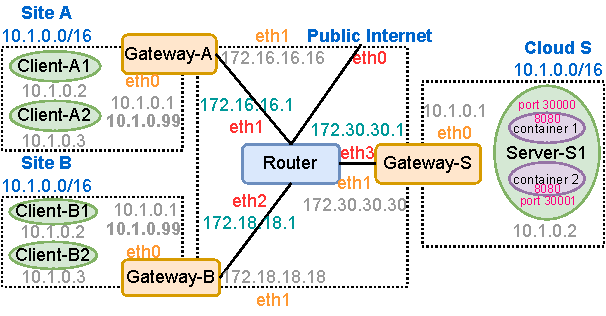
\includegraphics[scale=1]{figures/host-to-host.pdf}
    \label{fig:host2host}
  \end{center}
\end{figure}
\end{frame}

\subsection{Site to Site in IPv6}
\begin{frame}{Site to Site in IPv6}
\begin{figure}[t!]
  \begin{center}
    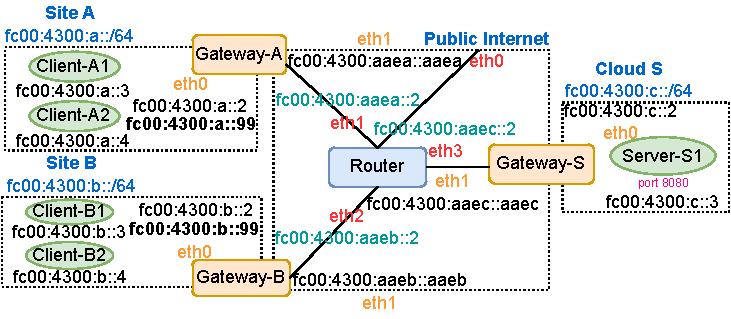
\includegraphics[scale=0.95]{figures/ipv6-site-to-site.pdf}
    \label{fig:ipv6site2site}
  \end{center}
\end{figure}
\end{frame}

\section{Evaluation}
\subsection{Usability and Portability}
\begin{frame}{Usability and Portability}
With \textbf{Docker Compose}, the Docker orchestration tool, containers \textbf{outperforms} VirtualBox-based Vagrant in many aspects:
\begin{table}[t!]
  \begin{center}
    \caption{Functionalities Comparison}
    \begin{tabular}{|l|c|c|}
    \hline
    \textbf{Items} & \textbf{Vagrant + VirtualBox} & \textbf{Docker Compose} \\
    \hline
    \textbf{Resources} & Heavy & Lightweight \\
    \hline
    \textbf{Kernel} & Own & Shared (Namespaces)\\
    \hline
    \textbf{Scalability} & Hard & Easy \\
    \hline
    \textbf{M1/M2 Support} & Limited & Fully \\
    \hline
    \textbf{Image Hub} & Unavailable & Available (Docker Hub) \\
    \hline
    \textbf{Seamless} & No & Yes \\
    \hline
    \end{tabular}
    \label{tab:compare}
  \end{center}
\end{table}
\end{frame}

\subsection{Performance}
\begin{frame}{Performance}
    Table below shows the metrics for the performance evaluation:
    \begin{table}[t!]
      \begin{center}
        \caption{Performance Test Result in Average}
        \begin{tabular}{|l|lr|}
        \hline
        Solution               & Boot Time$^1$ & Memory$^2$ \\
        \hline
        Docker Compose         &   75 s    &  278 MB \\
        Vagrant + VirtualBox   &  689 s    &  4.5 GB \\
        \hline
        \end{tabular}
        \label{tab:result}
      \end{center}
    \end{table}
    The container based solution \textit{reduces}:
    \begin{enumerate}
    \item \textbf{Fresh boot time}\footnote{Also include the running environment building time for the host platform} by nearly \textit{90\%}
    \item \textbf{Memory consumption}\footnote{Maximum value during the whole running process} by nearly \textit{94\%}
    \end{enumerate}
\end{frame}

\subsection{Security and Limitations}
\begin{frame}{Security and Limitations}
\begin{itemize}
\item We can't visit the host network interfaces inside containers, and vice versa. The container network stacks are \textbf{isolated} from host.
\end{itemize}

\begin{itemize}
\item Limitations of the Docker networking model include:
\begin{enumerate}
\item Disallowing to assign \textbf{overlapped IP address ranges} by Docker, even for network interfaces that won't directly connected.
\item Disallowing to assign \textbf{IP address ending in ".1"} by Docker, as these addresses are reserved by Docker for gateways or routers.
\end{enumerate}
\item However, we can always choose to configure the IP addresses manually inside containers to bypass these limitations.
\end{itemize}
\end{frame}

\section{Conclusion}
\begin{frame}{Conclusion}
\begin{itemize}
\item Containers are much more \textbf{lightweight} than virtual machines.
\item As a mature virtualization technology, containers can \textbf{realize every functionality} we require for virtual network systems.
\item Container is a suitable \textbf{replacement} for virtual machines if you want to migrate the virtual network systems away from VMs.
\item Hope it can inspire researchers and engineers to migrate their network systems testing environment from VMs into containers.
\end{itemize}
\end{frame}

\section{Q\&A}
\begin{frame}{Q\&A}
\centering
\huge{\textbf{Thanks for listening!}}

Any Questions?
\begin{figure}[t!]
  \begin{center}
    
\includegraphics[scale=0.075]{slide/img/source.png}
    \caption{Scan to get the case study implementation source code}
    \label{fig:source}
  \end{center}
\end{figure}
\end{frame}
\end{document}
